\section{LASSO}
%%%%%%%%%%%%%%%%%%%%%%%%%%%%%%%%%%%%%%%%%%%%%%%%%%%%%%%%
\begin{frame}
  \frametitle{Least Absolute Shrinkage and Selection Operator (LASSO)}
  \framesubtitle{B\"{u}hlmann \& van de Geer (2011); Hastie, Tibshirani \& Wainwright (2015)}

  Assume that $X$ has been centered: don't penalize intercept!

  \begin{block}{Notation}
    $\left| \left| \beta\right| \right|_2^2 = \sum_{j=1}^p \beta_j^2, \quad \left| \left| \beta\right| \right|_1 = \sum_{j=1}^p |\beta_j|$
  \end{block}

  \begin{block}{Ridge Regression -- $L_2$ Penalty}
	$\widehat{\beta}_{Ridge} =\underset{\beta}{\arg \min}\; (\mathbf{y} -  X\beta)' (\mathbf{y} - X\beta) + \lambda \left| \left| \beta\right| \right|_2^2$
  \end{block}

  \begin{block}{LASSO -- $L_1$ Penalty}
	$\widehat{\beta}_{Lasso} =\underset{\beta}{\arg \min}\; (\mathbf{y} - X\beta)' (\mathbf{y} - X\beta) + \lambda \left| \left| \beta\right| \right|_1$
  \end{block}

  
\end{frame}
%%%%%%%%%%%%%%%%%%%%%%%%%%%%%%%%%%%%%%%%%%%%%%%%%%%%%%%%
\begin{frame}
  \frametitle{Other Ways of Thinking about LASSO}
  \begin{block}{Constrained Optimization}
	$\underset{\beta}{\arg \min} (\mathbf{y}  - X\beta)' (\mathbf{y} - X\beta) \quad \mbox{subject to}\quad \sum_{j=1}^p |\beta_j| \leq t$
Data-dependent, one-to-one mapping between $\lambda$ and $t$.
\end{block}

\begin{block}{Bayesian Posterior Mode}
    Ignoring the intercept, LASSO is the posterior model for $\beta$ under
		\[\mathbf{y}|X,\beta, \sigma^2 \sim N(X\beta,\sigma^2 I_n), \quad
    \beta\sim \prod_{j=1}^p \mbox{Lap}(\beta_j|0, \tau)\]
  where  
  $\lambda= 1/\tau$ and 
  $\mbox{Lap}(x|\mu,\tau)= (2\tau)^{-1}\exp\left \{-\tau^{-1}|x-\mu| \right\}$
\end{block}
\end{frame}
%%%%%%%%%%%%%%%%%%%%%%%%%%%%%%%%%%%%%%%%%%%%%%%%%%%%%%%%
\begin{frame}
  \frametitle{Comparing Ridge and LASSO -- Bayesian Posterior Modes}
    
\begin{figure}
	\centering
	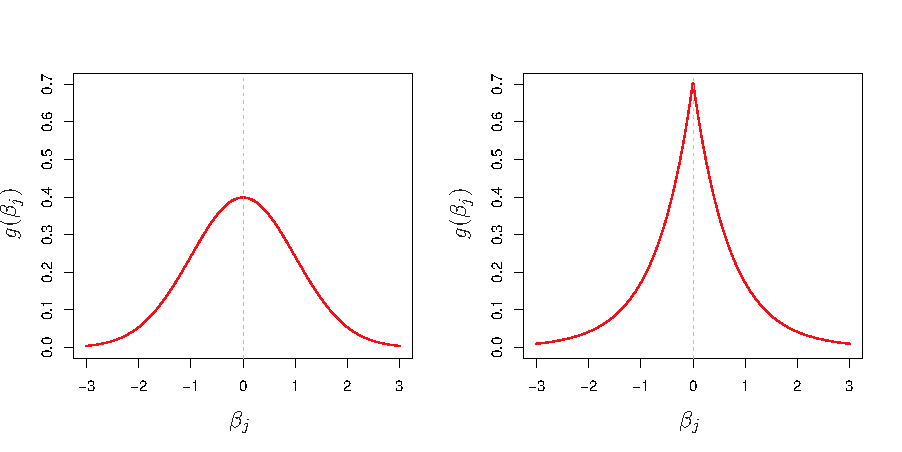
\includegraphics[scale=0.65]{../img/ISLR_ch6_fig11}
	\label{fig:ridge_lasso_prior}
  \caption{Ridge, at left, puts a normal prior on $\beta$ while LASSO, at right, uses a Laplace prior, which has fatter tails and a taller peak at zero.}
\end{figure}

\end{frame}
%%%%%%%%%%%%%%%%%%%%%%%%%%%%%%%%%%%%%%%%%%%%%%%%%%%%%%%%
\begin{frame}
  \frametitle{Comparing LASSO and Ridge -- Constrained OLS}
  
\begin{figure}
	\centering
	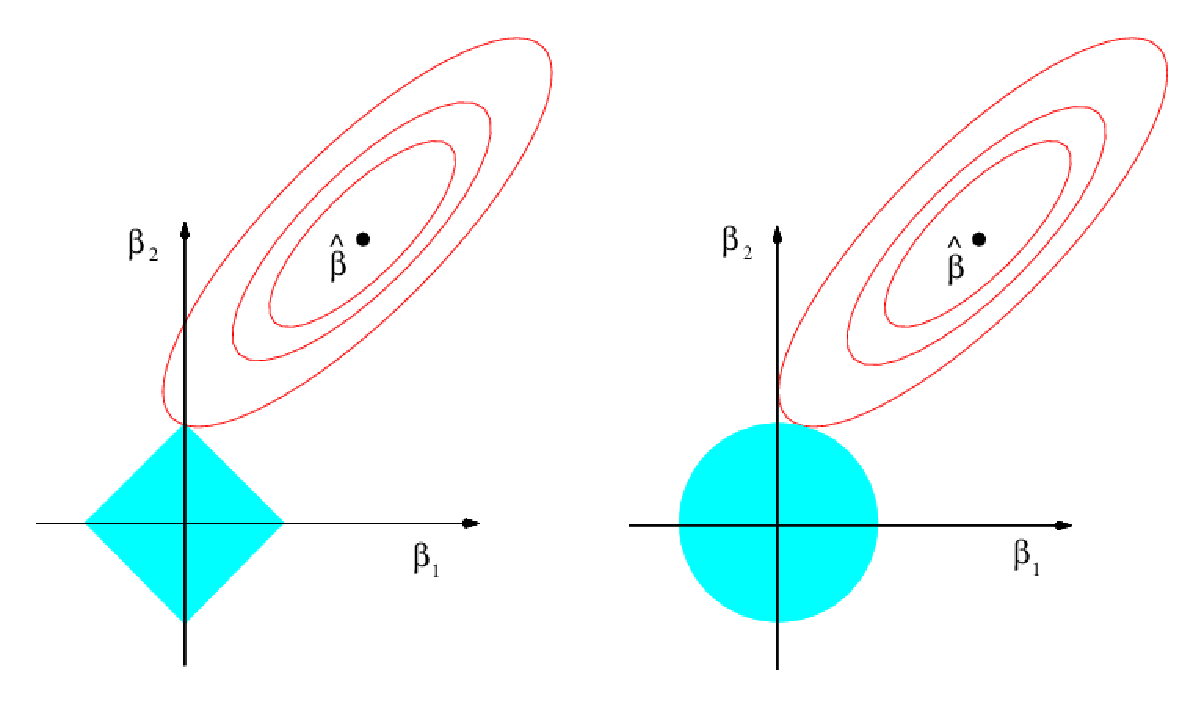
\includegraphics[scale=0.43]{../img/ISLR_ch6_fig7}
	\caption{$\widehat{\beta}$ denotes the MLE and the ellipses are the contours of the likelihood. 
LASSO, at left, and Ridge, at right, both shrink $\beta$ away from the MLE towards zero.
Because of its diamond-shaped constraint set, however, LASSO favors a \alert{sparse solution} while Ridge does not}
	\label{fig:ridge_lasso_constraint}
\end{figure}
\end{frame}
%%%%%%%%%%%%%%%%%%%%%%%%%%%%%%%%%%%%%%%%%%%%%%%%%%%%%%%%
\begin{frame}
  {No Closed-Form for LASSO!}

  \small

  \begin{block}{Simple Special Case}
  Suppose that $X'X = I_p$
\end{block}
\begin{block}{Maximum Likelihood}
    $\widehat{\boldsymbol{\beta}}_{MLE} = (X'X)^{-1}X'\mathbf{y} = X'\mathbf{y}, \quad \widehat{\beta}_j^{MLE} = \sum_{i=1}^n x_{ij}y_i$ 
  \end{block}

  \begin{block}{Ridge Regression}
    $\widehat{\boldsymbol{\beta}}_{Ridge} = (X'X + \lambda I_p)^{-1}X'\mathbf{y} = \left[ (1 + \lambda) I_p \right]^{-1} \widehat{\boldsymbol{\beta}}_{MLE},\quad \widehat{\beta}^{Ridge}_j = \displaystyle \frac{\widehat{\beta}^{MLE}_j}{1 + \lambda}$
  \end{block}

  \begin{alertblock}{So what about LASSO?}
  \end{alertblock}
\end{frame}
%%%%%%%%%%%%%%%%%%%%%%%%%%%%%%%%%%%%%%%%%%%%%%%%%%%%%%%%
\begin{frame}
  \frametitle{LASSO when $X'X= I_p$ so $\widehat{\beta}_{MLE} = X'\mathbf{y}$}

  \begin{block}{Want to Solve}
    \vspace{-1.5em}
    $$\widehat{\boldsymbol{\beta}}_{LASSO} = \underset{\boldsymbol{\beta}}{\arg \min}\; (\mathbf{y}  - X\boldsymbol{\beta})' (\mathbf{y} - X\boldsymbol{\beta}) + \lambda \left| \left| \boldsymbol{\beta}\right| \right|_1$$
  \end{block}

  \begin{block}{Expand First Term}
    \vspace{-1.5em}
	\begin{eqnarray*}
    (\mathbf{y}  - X\boldsymbol{\beta})' (\mathbf{y} - X\boldsymbol{\beta}) &=& \mathbf{y}'\mathbf{y} - 2\boldsymbol{\beta}' X' \mathbf{y} + \boldsymbol{\beta}' X'X \boldsymbol{\beta} \\
    &=& (\mbox{constant}) - 2\boldsymbol{\beta}' \widehat{\boldsymbol{\beta}}_{MLE} + \boldsymbol{\beta}'\boldsymbol{\beta}
	\end{eqnarray*}
  \end{block}

  \begin{block}{Hence}
    \vspace{-1.5em}
\begin{eqnarray*}
  \widehat{\boldsymbol{\beta}}_{LASSO} &=& \underset{\boldsymbol{\beta}}{\arg \min}\; (\boldsymbol{\beta}'\boldsymbol{\beta} - 2\boldsymbol{\beta}' \widehat{\boldsymbol{\beta}}_{MLE})  +  \lambda \left| \left| \boldsymbol{\beta}\right| \right|_1\\
  &=& \underset{\boldsymbol{\beta}}{\arg \min}  \sum_{j=1}^p \left(\beta_j^2 - 2 \beta_j \widehat{\beta}^{MLE}_j + \lambda\left|\beta_j \right|\right)
\end{eqnarray*}
    
  \end{block}
  
\end{frame}
%%%%%%%%%%%%%%%%%%%%%%%%%%%%%%%%%%%%%%%%%%%%%%%%%%%%%%%%
\begin{frame}
  \frametitle{LASSO when $X'X = I_p$}
  \begin{block}{Preceding Slide}
    \vspace{-1.5em}
\begin{eqnarray*}
  \widehat{\boldsymbol{\beta}}_{LASSO} 
  &=& \underset{\boldsymbol{\beta}}{\arg \min}  \sum_{j=1}^p \left(\beta_j^2 - 2 \beta_j \widehat{\beta}^{MLE}_j + \lambda\left|\beta_j \right|\right)
\end{eqnarray*}
  \end{block}

  \vspace{-1em}

  \begin{alertblock}{Key Simplification}
  Equivalent to solving $j$ independent optimization problems:
  \vspace{-0.5em}
  \[
	\widehat{\beta}^{Lasso}_j = \underset{\beta_j}{\arg \min} \left(\beta_j^2 - 2 \beta_j \widehat{\beta}^{MLE}_j + \lambda\left|\beta_j \right|\right)
  \]
  \vspace{-2em}
  \begin{itemize}
    \item Sign of $\beta_j^2$ and $\lambda |\beta_j|$ unaffected by $\mbox{sign}(\beta_j)$
    \item $\widehat{\beta}_j^{MLE}$ is a function of data only -- outside our control
    \item Minimization requires \alert{matching} $\mbox{sign}(\beta_j)$ to $\mbox{sign}(\widehat{\beta}^{MLE}_j)$
  \end{itemize}
  \end{alertblock}
\end{frame}
%%%%%%%%%%%%%%%%%%%%%%%%%%%%%%%%%%%%%%%%%%%%%%%%%%%%%%%%
\begin{frame}
  \frametitle{LASSO when $X'X = I_p$}

  \begin{block}{Case I: $\widehat{\beta}^{MLE}>0 \implies \beta_j > 0 \implies |\beta_j| = \beta_j$}
    
Optimization problem becomes
\[\widehat{\beta}^{Lasso}_j = \underset{\beta_j}{\arg \min} \; \beta_j^2 - 2 \beta_j \widehat{\beta}^{MLE}_j + \lambda\beta_j\]
Interior solution:
\[\widehat{\beta}_j = \widehat{\beta}^{MLE}_j - \frac{\lambda}{2}\]
  Can't have $\beta_j<0$: corner solution sets $\beta_j = 0$
\[\widehat{\beta}^{Lasso}_j = \max\left\{0,\widehat{\beta}^{MLE}_j - \frac{\lambda}{2}\right\}\] 
  \end{block}
  
\end{frame}
%%%%%%%%%%%%%%%%%%%%%%%%%%%%%%%%%%%%%%%%%%%%%%%%%%%%%%%%
\begin{frame}
  \frametitle{LASSO when $X'X = I_p$}

  \begin{block}{Case II: $\widehat{\beta}^{MLE}\leq0 \implies \beta_j \leq 0 \implies |\beta_j| = -\beta_j$}
    
Optimization problem becomes
\[\widehat{\beta}^{Lasso}_j = \underset{\beta_j}{\arg \min} \; \beta_j^2 - 2 \beta_j \widehat{\beta}^{MLE}_j - \lambda\beta_j\]
Interior solution:
\[\widehat{\beta}_j = \widehat{\beta}^{MLE}_j + \frac{\lambda}{2}\]
  Can't have $\beta_j>0$: corner solution sets $\beta_j = 0$
\[\widehat{\beta}^{Lasso}_j = \min\left\{0,\widehat{\beta}^{MLE}_j + \frac{\lambda}{2}\right\}\] 
  \end{block}
  
\end{frame}
%%%%%%%%%%%%%%%%%%%%%%%%%%%%%%%%%%%%%%%%%%%%%%%%%%%%%%%%
\begin{frame}
  \frametitle{Ridge versus LASSO when $X'X = I_p$}
\begin{figure}
	\centering
	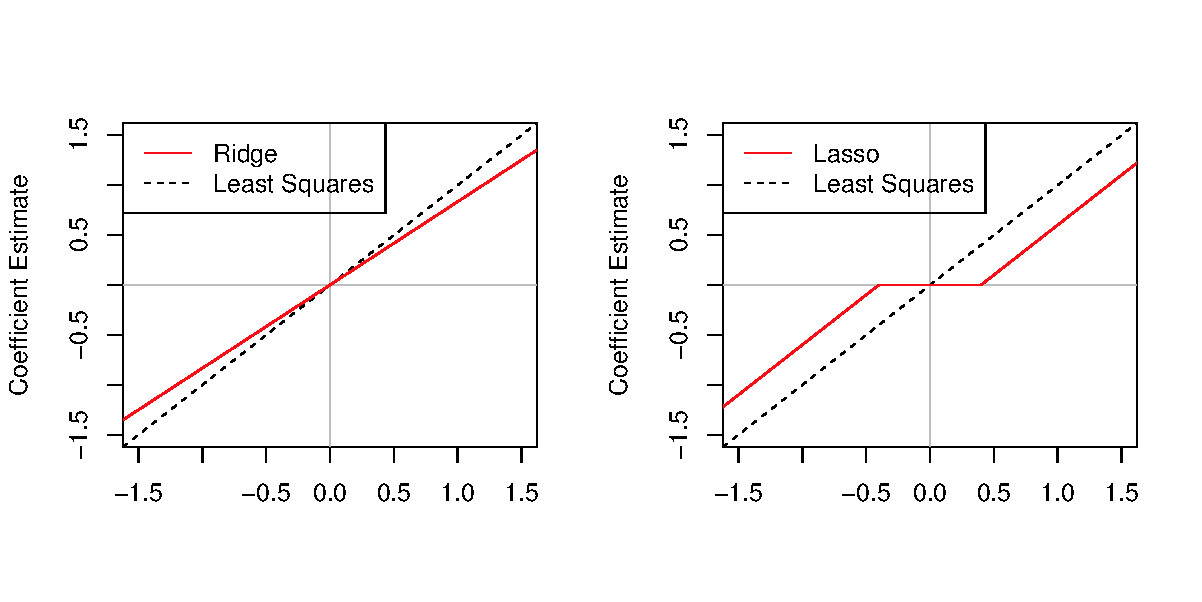
\includegraphics[scale=0.5]{../img/ISLR_ch6_fig10}
	\caption{Horizontal axis in each plot is MLE}
\end{figure}

\vspace{-3em}
	\begin{eqnarray*}
		\widehat{\beta}^{Ridge}_j &=&  \left(\frac{1}{1+\lambda}\right)\widehat{\beta}^{MLE}_j\\
    \widehat{\beta}^{Lasso}_j &=&\mbox{sign}\left(\widehat{\beta}^{MLE}_j \right)\max\left\{0, \left| \widehat{\beta}^{MLE}_j\right| - \frac{\lambda}{2} \right\}
	\end{eqnarray*}
\end{frame}
%%%%%%%%%%%%%%%%%%%%%%%%%%%%%%%%%%%%%%%%%%%%%%%%%%%%%%%%
\begin{frame}
  \frametitle{Calculating LASSO -- The Shooting Algorithm}
  \framesubtitle{Cyclic Coordinate Descent}

  \begin{algorithm}[H]
    \KwData{$\mathbf{y}$, $X$, $\lambda\geq 0$, $\varepsilon > 0$} 
  \KwResult{LASSO Solution}

  $\boldsymbol{\beta} \leftarrow \mbox{ridge}(X, \mathbf{y}, \lambda)$
 

  \Repeat{$\sum_{j=1}^p |\beta_j^{prev} - \beta_j|< \varepsilon$}{
    $\boldsymbol{\beta}^{prev} \leftarrow \boldsymbol{\beta}$

   \For{$j = 1, \dots, p$}{
     $a_j \leftarrow 2 \sum_{i=1}^n x_{ij}^2$

     $c_j \leftarrow 2\sum_{i=1}^n x_{ij}(y_i - \mathbf{x}_i' \mathbf{\beta} + \beta_j x_{ij})$

     $\beta_j \leftarrow \mbox{sign}(c_j/a_j) \max \left\{0, |c_j/a_j| - \lambda/a_j \right\}$ 

   }}
\end{algorithm}

\end{frame}
%%%%%%%%%%%%%%%%%%%%%%%%%%%%%%%%%%%%%%%%%%%%%%%%%%%%%%%%
